\documentclass[11pt]{article}
\usepackage{amsmath}
\usepackage{amssymb}
\usepackage{fancyhdr}
\usepackage{graphicx}
\usepackage{pdfpages}
\usepackage{listings}
\usepackage{color}
\usepackage{color}
\usepackage{lmodern}
\definecolor{dkgreen}{rgb}{0,0.6,0}
\definecolor{gray}{rgb}{0.5,0.5,0.5}
\definecolor{mauve}{rgb}{0.58,0,0.82}
\pagestyle{headings}
\setlength{\oddsidemargin}{0in}
\setlength{\evensidemargin}{0in}
\setlength{\textheight}{9in}
\setlength{\textwidth}{6.5in}
\setlength{\topmargin}{-0.5in}
\setlength{\headheight}{14pt}
\renewcommand*\rmdefault{lmss}
\renewcommand*\contentsname{Table of Contents}
\lstset{language=R,
	aboveskip=3mm,
	belowskip=3mm,
	showstringspaces=false,
	%basicstyle={\small\ttfamily},
	basicstyle={\normalfont\ttfamily},
	numbers=left,
	numberstyle=\tiny\color{gray},
	keywordstyle=\color{blue},
	commentstyle=\color{dkgreen},
	stringstyle=\color{mauve},
	breaklines=true,
	breakatwhitespace=true,
	tabsize=4
}

%%%%%%%%%%%%%%%%%%%%%%%%%%%%%
\title{\vspace{-3ex}\bf Final Project\\[2ex] 
       \normalsize ECS 132 --- Winter 2015}
\date{\today}
\author{\bf William Otwell (997371020)\\ \bf Rupali Saiya (997286348)\\ \bf Nicholas Layton(996933702)\\ \bf Syeda Inamdar(997323599)\\}

\begin{document}
\maketitle
\pagebreak
\tableofcontents
\pagebreak

%%%%%%%%%%%%%%%%%%%%%%%%%%%%%
\section{Problem 1}
\label{sec:problem1}
\subsection{Part A: Comparison of Two Means}
\label{subsec:1a}
The bike sharing dataset provided by the UC Irvine (UCI) Machine Learning Repository allows us to analyze bike rental statistics during the years 2011 and 2012. We decided to analyze and compare the quantity of bike rentals on days during the months of March 2011 and March 2012 to gain insight as to how much the bike rental rates changed from one year to the next. In more formal terms, we estimated the difference between the average number of bikes rented in March 2011 and the average number of bikes rented in March 2012. To do so, we constructed a confidence interval from the sample provided by UCI to estimate the difference between the population means of the averages from each month. We first had to define our random variables before constructing our confidence interval. Below is a list of the random variables that we used:
\begin{itemize}
	\item $X$: the number of bikes rented on any given day in March 2011
	\item $Y$: the number of bikes rented on any given day in March 2012
	\item $\bar{X}$: the sample mean of the number of bikes rented per day in March 2011
	\item $\bar{Y}$: the sample mean of the number of bikes rented per day in March 2012
	\item $s_1$: the standard deviation of the number of bikes rented per day in March 2011
	\item $s_2$: the standard deviation of the number of bikes rented per day in March 2012
\end{itemize}
An important aspect worth noting is that the random variables $X$ and $Y$ are independent of one another. After defining our random variables, we had to construct our model for constructing the confidence interval. Our model turned out to be the following:
\begin{equation}
\bar{X} - \bar{Y} \pm (1.96) \sqrt{\frac{s_{1}^{2}}{n_1} + \frac{s_{2}^{2}}{n_2}}
\end{equation}
\dots where $n_1$ and $n_2$ were the number of days in March 2011 and March 2012 (respecfully) for which data was recorded. The R code that we developed to calculate this confidence interval can be found in Appendix~\ref{sec:problem1code}.

After running our R calculations, we found that the average number of bike rentals in March 2011 was 2065.968 bikes and that of March 2012 was 5318.548 bikes. The difference between the means of our two samples was -3252.581. The standard deviation of the number of bikes rented in March 2011 was 550.9717, and the standard deviation of that in March 2012 was 1251.1627. From these values, we found our confidence interval to be $(-5932.108, -573.0535)$. In formal terms, we are 95\% confident that the difference between the mean number of bike rentals on days in March 2011 and days in March 2012 lies within the interval ranging from $-5932.108$ to $-573.0535$.  

Although this is a very wide ranging interval, we still were able to make inferences about the bike rental trends in March 2011 versus the trends in March 2012. Being that we subtracted the sample mean of the bike rentals in March 2012 from that of the bike rentals in March 2011, we inferred that there were significantly more bike rentals in March 2012 than there were in March 2011. This is because the entirety of the interval lies below 0. In the next section, we used a proportion of warmer days in the same two months to see if temperature could have influenced the increase in the number of bike rentals from March 2011 to March 2012.

\subsection{Part B: Comparison of Two Proportions}
\label{subsec:1b}
We wanted to compare the proportion of warmer than average days in March 2011 to those in March 2012. We constructed a confidence interval to estimate the difference between population proportions of the number of warmer days in March 2011 and March 2012. Again, we defined our random variables and then constructed the confidence interval. 
\begin{itemize}
	\item $\hat{p_1}$: the sample proportion of warmer days in March 2011
	\item $\hat{p_2}$: the sample proportion of warmer days in March 2012
	\item $s_{1}^{2}$: the standard deviation of the proportion of warmer days in March 2011
		\subitem Mathematical expression: $s_{1}^{2} =\hat{p_1}(1 - \hat{p_1})$
	\item $s_{2}^{2}$: the standard deviation of the proportion of warmer days in March 2012
		\subitem Mathematical expression: $s_{2}^{2} = \hat{p_2}(1 - \hat{p_2})$
\end{itemize}
The random variables $\hat{p_1}$ and $\hat{p_2}$ are independent of one another. The model that we used to calculate the confidence interval for the difference in the two proportions was:
\begin{equation}
\hat{p_1} - \hat{p_2} \pm (1.96) \sqrt{\frac{s_1^2}{n_1}+\frac{s_2^2}{n_2}} 
\end{equation}
\begin{equation}
= \hat{p_1} - \hat{p_2} \pm (1.96) \sqrt{\frac{\hat{p_1}(1 - \hat{p_1})}{n_1}+\frac{\hat{p_1}(1 - \hat{p_1})}{n_2}}
\end{equation}
\dots where $n_1$ and $n_2$ are the number of days in March 2011 and March 2012 (respectfull) during which the temperature was warm. We defined a "warmer day" to be one in which the temperature rose above 12.5 degrees Celsius, which translated to be 0.3 in the UCI dataset. The R code that was developed to evaluate the above expression can be found in Appendix~\ref{sec:problem1code}.

In our calculation we found that the proportion of warmer days in March 2011 was 0.5806452 and that the proportion of warmer days in March 2012 was 0.9032258. The difference between the proportions of our two samples was found to be 0.3225833. The standard deviation of the proportion of warmer days in March 2011 was 0.4934535, and the standard deviation of the proportion of warmer days in March 2012 was 0.2956500. The resulting confidence interval was $(-0.5250816, -0.1200797)$. We can say that we are 95\% confident that the difference between the population proportions for warmer days in the months of March 2011 and March 2012 lies within the interval ranging from $-0.5250816$ to  $-0.1200797$.

These two confidence intervals show that there could be a relationship between the proportion of warmer days and the number of bike rentals in the month of March. We can see that both the proportion of warmer days and the number of bike rentals in March 2012 were greater than that of March 2011, which suggests that warmer weather could have influenced more people to rent bikes. Although it makes intuitive sense that there is a relationship between warmer weather and an increase in bike rentals, our calculations cannot ensure that warmer weather was, in fact, the reason why there were more people renting bikes. We can only say that there is a potential relationship, given that the confidence intervals indicate as such. 
\pagebreak



%%%%%%%%%%%%%%%%%%%%%%%%%%%%%
\section{Problem 2}
\label{sec:problem2}
\subsection{Part A}
\label{subsec:2a}
In this part we realized that casual, registered and dtedate were not necessary to include as predictors.
\subsection{Part B}
\label{subsec:2b}
Please see Appendix~\ref{sec:problem2code} for the code from Part B. Part C and D will explore the output of this code in detail.   
\subsection{Part C}
\label{subsec:2c}

When we fit a linear model on our training data set, the output returned is our sample estimate (estimate based on our sample data). The output that was returned is included in the Appendix~\ref{sec:problem2coutput}.
\\

The first coefficient returned is the intercept value, which we can call $\beta_{0}$. The estimates for our next 11 coefficients returned are our predictors, which we can call  $\beta_{i}$, where i is a number 1 through 11. These values can help us estimate average bike ridership from our sample data. The linear model of our estimated regression would be:
\begin{equation}
\text{mean count} = \beta_0 + \beta_1 \text{season} + \beta_2 \text{yr} + \beta_3\text{mnth} + \beta_4\text{holiday} + \beta_5\text{weekday} + \beta_6\text{workingday} +  \dots
\end{equation}
\begin{equation}
\dots \beta_7 \text{weathersit} + \beta_8 \text{temp} + \beta_9 \text{atemp} + \beta_{10} \text{hum} + \beta_{11} \text{windspeed}
\end{equation}

The above just gives a sample estimate, it is not representative of the population bike ridership function. Looking at the estimate values for the coefficients one can see that we have positive and negative values. The coefficients that have negative values indicate attributes that result in a decrease of bike ridership. For example, the estimate for holidays is -380.192. This makes sense because bike ridership would decrease if it is a holiday as most people would be out of town or with their families in our sample. The coefficients that have positive values indicate attributes that result in an increase of bike ridership. For example, the estimate for temp is 487.505, which indicates that as the temperature increases (gets warmer) there is more bike ridership on average in our sample.  

To get an idea of how accurate our estimate is, we can use the standard error of each of $\beta_i$ to calculate a 95\% confidence interval. This will tell us that we are 95\% confident that the true predictor for that particular coefficient is in that interval. The R-squared value tells us that we can predict bike ridership from these eleven coefficients about 76.31\% of the time. 

\subsection{Part D}
\label{subsec:2d}
We have added two interaction terms and one quadratic term to the linear model. Our output can be viewed in Appendix~\ref{sec:problem2doutput}. The interaction terms are temp and workingday. We multiplied temp and workingday with the -1127.08 result from the linear model to demonstrate that with higher temperatures on a workingday, the number of bike rentals decreases. The other interaction terms are  mnth and weathersit. We multiplied mnth and weathersit to indicate later months coupled with poor weather leads to a decreased number of bike rentals. Our quadratic term tempsquared is used to emphasize the fact that as the temperature increases, there are less bike rentals.  
Compared to part C, our R-squared value is now 81.73\% which demonstrates that this model is a more accurate representation of our sample estimate. 
\subsection{Part E}
\label{subsec:2e}
Our final model included the following attributes: year (yr), temp, humidity (hum), windspeed,tempsquared, spring, summer, fall, raining. Tempsquared is the temp values squared. We chose to do this so that we could place more emphasis on the days that had warmer weather because that seems to be a very large contributing factor to bike ridership. In addition, we decided to break the seasons into spring, summer, and fall because the boolean values for season were being incorporated into the original model. For example, fall was flagged as a 3. In  the original model, that 3 would be carried into the calculations. By adding these new attributes, we can now make spring, summer, and fall a boolean 1 or 0 so the calculations are not skewed. Although we are only tracking spring, summer, and fall values, we can assume if the value is not one of the three it is winter. Therefore, we can use these values to compare against winter. Lastly, the raining attribute compares weather situations 1 and 2 against 3 and 4 (clear and misty vs. light and heavy rain). We chose to exclude the workingday, weekend, weekday, and holiday attributes because we saw these items did not impact bike ridership.

\subsection{Part F}
\label{subsec:2f}
The output that R returned to us is in Appendix~\ref{sec:problem2efoutput}. The first indication that this model is more accurate than our previous models is that our R-square value is now approximately 0.8436. This shows that we can accurately predict 84.36\% of biker ridership for our sample. We also print out the mean, min and max of the difference between value that was predicted by the regression and the actual value of the validation set. The average difference between our prediction and validation data was approximately 573.579. We ran our model multiple times with different attributes to gage whether this difference in mean would increase or decrease, and found this average difference to be among the lower values. 
\subsection{Part G}
\label{subsec:2g}
\subsection{Part H}
\label{subsec:2h}
\pagebreak

%%%%%%%%%%%%%%%%%%%%%%%%%%%%%
\section{Problem 3}
\label{sec:problem3}
\subsection{Part A: Nonparametric Density Estimation}
\label{subsec:3a}


\subsection{Part B: Fitting a Parametric Model}
\label{subsec:3b}
In the previous section, we formed a nonparametric estimate of the density of the daily temperature data by constructing a histogram. After analyzing the histogram, we chose to model its density with a normal parametric distribution. The histogram showed two peaks: one peak among the values that represented colder weather and another among those of warmer temperatures. It also showed a dip among values that are somewhere between colder and warmer temperatures. These observations suggested that the daily temperature from 2011 to 2012 in Washington D.C. matched that of a bimodal distribution, however, we theorized that the population temperature, in fact, could have been normally distributed.  

We thought that the frequency of days in which temperature was either extremely cold or extremely warm should be less than that of days in which the temperature was somewhere in between. Our theory came from the idea that climates seem to rarely shift from hot to cold (or vice-versa) in short periods of time, meaning there should be an extended period of time between these periods in which the weather is of moderate temperature. For this reason, we thought there should be a larger number of days of moderate temperature, and that the data should have represented a more normal distribution. 

In the following sections we explain how we fitted our data to a normal parametric model using two different approaches: the Method of Moments approach, and the Maximum Likelihood approach. 
\subsubsection{Method of Moments}
\label{subsubsec:methodofmoments}
The method of moments involves equation population parameters for a particular parametric distribution to its population moments. In the case of the normal distribution these parameters are the mean and the variance. To accurately fit the normal parametric model to our data, we had to determine the method of moments estimators for the mean and variance. We found the first and second theoretical moments to be: 
\begin{equation}
E(X_i) = \mu\ \ \&\ \ E(X_i^2) = \sigma ^ 2 + \mu ^ 2
\end{equation}
The second equation came from manipulating the formula for variance. We cam up with two equations to estimate the moments based on our sample data:
\begin{equation}
E(X_i) = \mu = \frac{1}{n} \sum_{i=1}^n X_i
\end{equation}
\begin{equation}
E(X_i^2) = \sigma ^ 2 + \mu ^ 2 = \frac{1}{n} \sum_{i=1}^{n} X_i^2
\end{equation}
We were able to calculate these values from our sample data of daily temperatures using R. The code that we developed to calculate these moments can be found in Appendix~\ref{sec:problem3code} in the function labeled "PartB()". From our code we determined the method of moments estimator for $E(X)$ to be .4953848 and the estimator for $E(X_i^2)$ to be .2788679 and therefore calculated the variance, $\sigma^2$, to be 0.030473 and the standard deviation, $\sigma$, to be 0.174565. We then used these estimated parameters in our function labeled "PartC()" to get an accurate fit to the data.
 
\subsubsection{Method of Maximum Likelihood}
\label{subsubsec:maximumlikelihood}
The method of maximum likelihood is a more commonly used method to find the likelihood (the probability) of our data values occurring. In the case of our normal distribution, the parameters are mean and standard deviation. To accurately fit the normal parametric model to our data, we had to determine the method of maximum likelihood estimators for the mean and standard deviation. The first step to find the estimators was to determine the likelihood function in terms of the product of the density values. We determined this to be:
\begin{equation}
L=\Pi_{i=1}^{n}\dfrac{1}{\sqrt{2\pi\sigma^2}}e^{-(x_i-\mu)^2/(2\sigma^2)}
\end{equation}
We can simplify this equation into:
\begin{equation}
L=(2\pi\sigma^2)^{-n/2}e^{-\dfrac{1}{2\sigma^2}\sum_{i}(x_i-\mu)^2}
\end{equation}

However, it is usually easier to maximize the log likelihood of a normal distribution. We determined this to be:
\begin{equation}
l(\mu,\sigma) = -\frac{n}{2}log(2\pi) - nlog(\sigma) - \frac{1}{2\sigma^{2}}\sum_{i}(x_i-\mu^2)
\end{equation} 

From here we were able to calculate the values from our sample data of daily temperature using R's mle() function. The code that we developed to calculate these moments can be found in Appendix~\ref{sec:problem3code} in the function labeled "PartB()". From our code we determined the method of maximum likelihood estimator for the mean, $\mu$, to be .4953848 and the estimator for the standard deviation, $\sigma$, to be .1829285. 


\subsection{Part C: Plotting Parametric-Model Curves}
\label{subsec:3c}
We plotted our two parametric model curves on top of the nonparametric density estimation (histogram), and found them to both be very similar. The calculated values of $\mu$ and $\sigma$ were very similar between the Method of Moments and the Method of Maximum Likelihood. In Appendix~\ref{sec:problem3plots} you can find our plots for Method of Moments and Method of Maximum Likelihood superimposed on our plot from "Part A()". The parametric curve for Method of Moments in Appendix~\ref{subsesc:problem3moments} is drawn in red and the curve for Method of Maximum Likelihood in Appendix~\ref{subsesc:problem3cmaximumlikelihood} is drawn in blue. The graph of Appendix~\ref{subsesc:problem3ccombined} shows a curve in purple, which includes the plot of Method of Moments and Method of Maximum Likelihood and shows us that both these methods calculated the same mean and standard deviations for the normal distribution.

\pagebreak

%%%%%%%%%%%%%%%%%%%%%%%%%%%%%
\appendix
\section{Problem 1 Code}
\label{sec:problem1code}
\lstinputlisting{Problem1.R}
\pagebreak

%%%%%%%%%%%%%%%%%%%%%%%%%%%%%
\section{Problem 2 Code}
\label{sec:problem2code}
\lstinputlisting{Problem2.R}
\pagebreak

%%%%%%%%%%%%%%%%%%%%%%%%%%%%%
\section{Problem 2 Output}
\label{sec:problem2output}
\subsection{Part C}
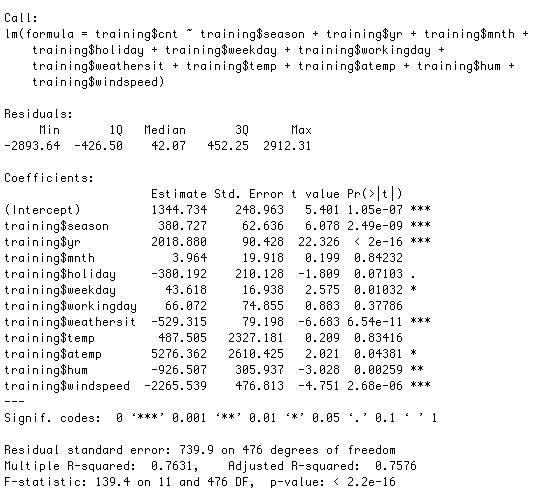
\includegraphics[totalheight=0.65\textheight]{Output.jpg}
\label{sec:problem2coutput}
\subsection{Part D}
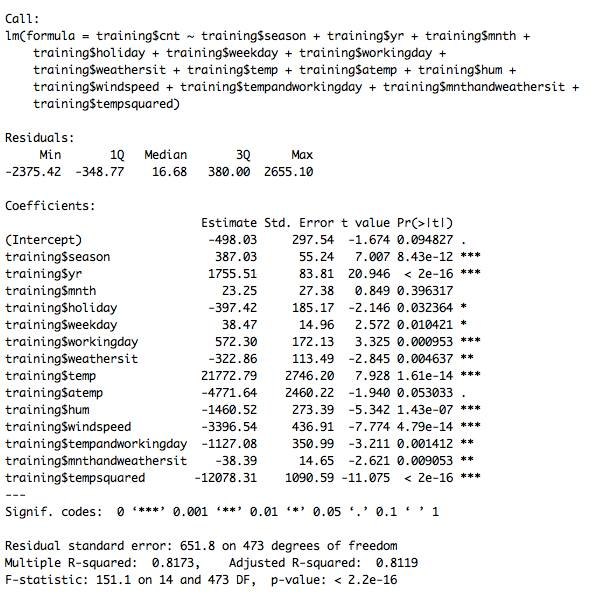
\includegraphics[totalheight=0.65\textheight]{Part2Doutput.jpg}
\label{sec:problem2doutput}
\pagebreak
\subsection{Part E and F}
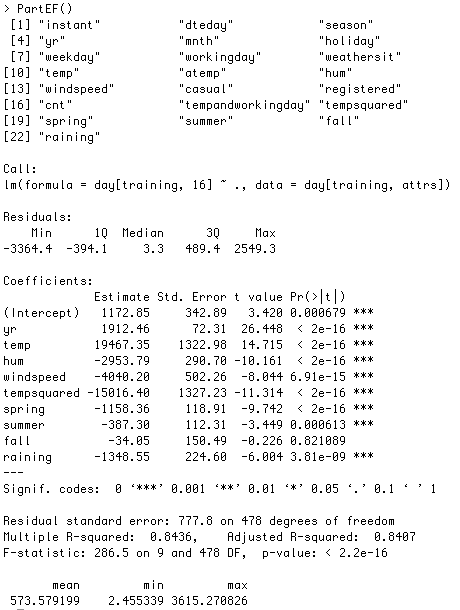
\includegraphics{Output2PartEF.jpg}
\label{sec:problem2efoutput}
\pagebreak
%%%%%%%%%%%%%%%%%%%%%%%%%%%%%
\section{Problem 3 Code}
\label{sec:problem3code}
\lstinputlisting{Problem3.R}
\pagebreak

%%%%%%%%%%%%%%%%%%%%%%%%%%%%%
\section{Problem 3 Plots}
\label{sec:problem3plots}
\subsection{Part A}
The plot below is the nonparametric estimate of our data set for daily temperatures. 
\newline
\label{sec:problem3aplot}
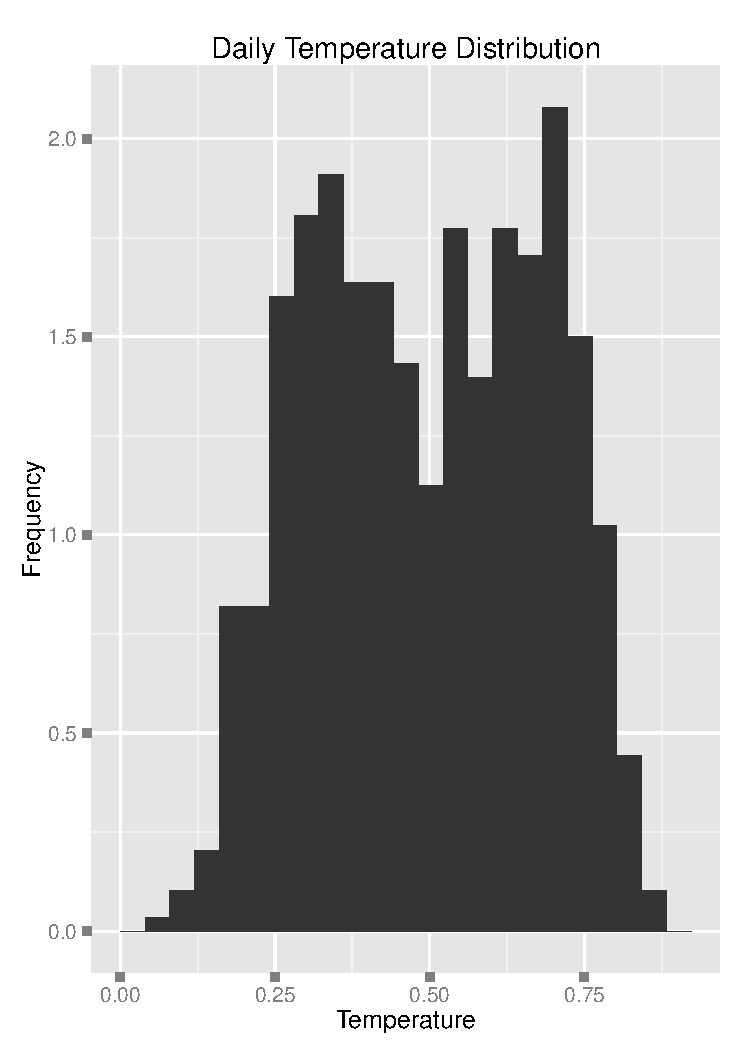
\includegraphics{Problem3A.pdf}
\newline
\pagebreak

\subsection{Part C: Method of Moments}
\label{subsesc:problem3moments}
The plot below is the parametric estimate of our data set for daily temperatures while using the Method of Moments approach to estimating the population parameters for a Normal Distribution. 
\newline
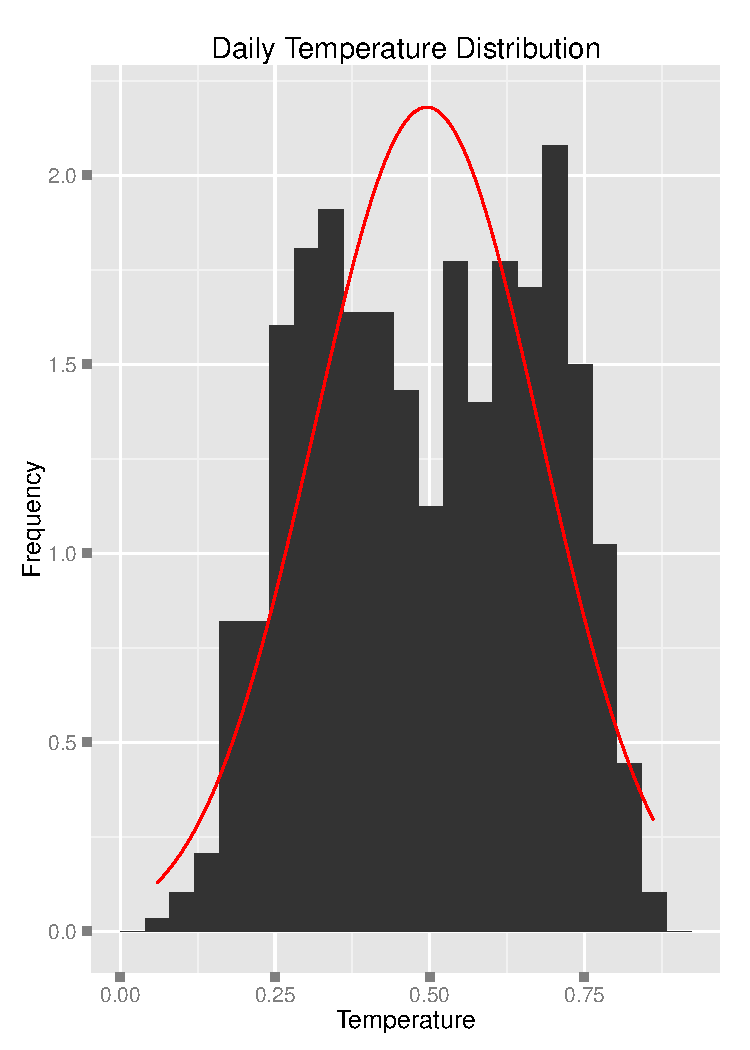
\includegraphics{Problem3CMoments.pdf}
\newline
\pagebreak

\subsection{Part C: Maximum Likelihood}
\label{subsesc:problem3cmaximumlikelihood}
The plot below is the parametric estimate of our data set for daily temperatures while using the Method of Maximum Likelihood to estimate the population parameters for a Normal Distribution. 
\newline
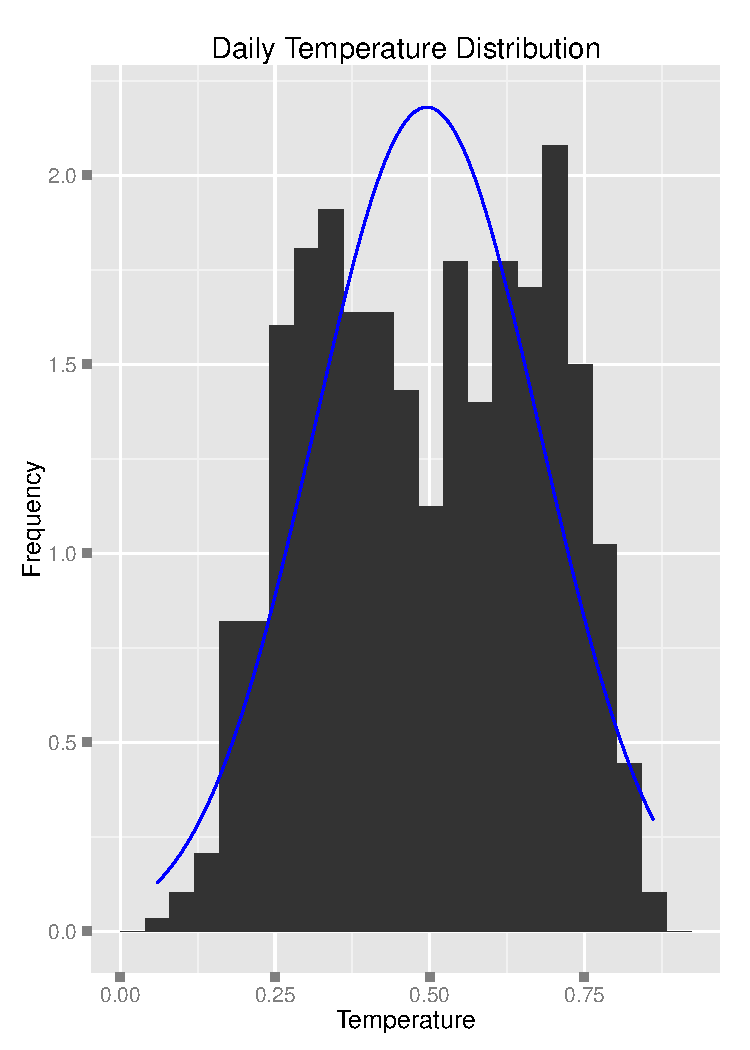
\includegraphics{Problem3CMLE.pdf}
\newline
\pagebreak

\subsection{Part C: Combined}
\label{subsesc:problem3ccombined}
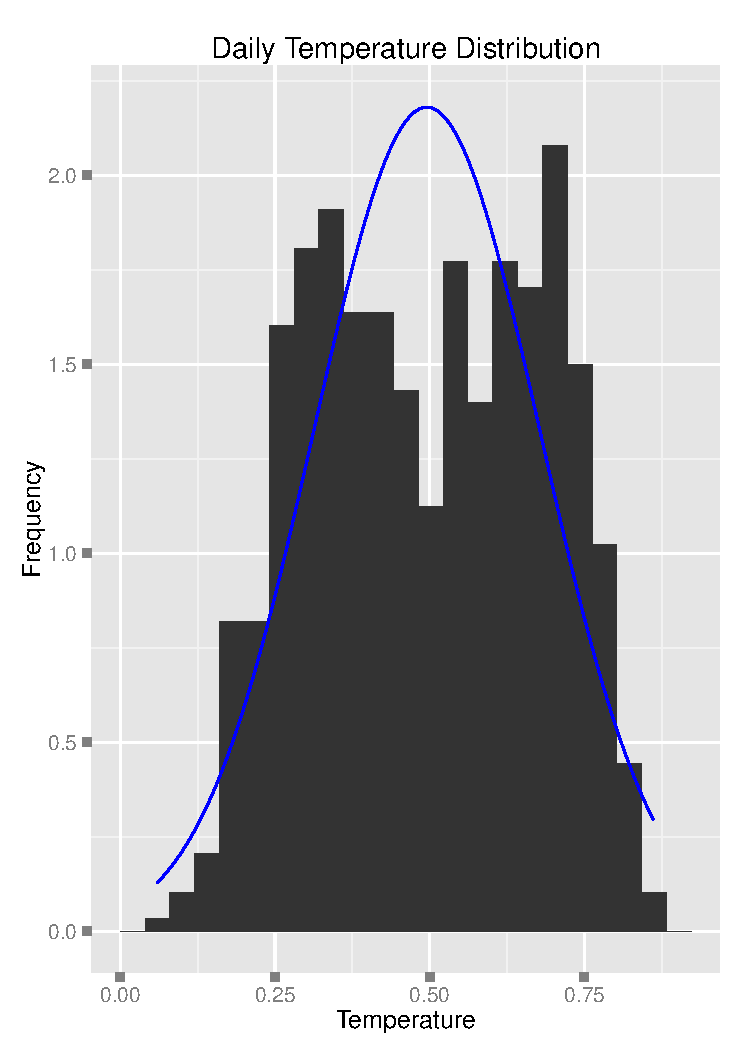
\includegraphics{Problem3C.pdf}
\newline
\pagebreak

%%%%%%%%%%%%%%%%%%%%%%%%%%%%%
\section{Group Member Contributions}
\begin{itemize}
	\item William Otwell:
	\begin{itemize}
		\item 
	\end{itemize}
	
	\item Rupali Saiya:
	\begin{itemize}
		\item 
	\end{itemize}
	
	\item Nicholas Layton:
	\begin{itemize}
		\item 
	\end{itemize}
	
	\item Syeda Inamdar:
	\begin{itemize}
		\item 
	\end{itemize}
\end{itemize}
\pagebreak

\end{document}

